\documentclass[11pt]{paper}
\usepackage{geometry}                % See geometry.pdf to learn the layout options. There are lots.
\geometry{letterpaper}                   % ... or a4paper or a5paper or ... 
%\geometry{landscape}                % Activate for for rotated page geometry
%\usepackage[parfill]{parskip}    % Activate to begin paragraphs with an empty line rather than an indent
\usepackage{graphicx}
\usepackage{amssymb}
\usepackage{epstopdf}
\usepackage{hyperref}
\usepackage{natbib}
\DeclareGraphicsRule{.tif}{png}{.png}{`convert #1 `dirname #1`/`basename #1 .tif`.png}

\newcommand{\aap}{{\it A\&A}}
%\newcommand{\aaps}{{\it A\&AS}}
\newcommand{\aj}{{\it AJ}}
\newcommand{\apj}{{\it ApJ}}
\newcommand{\apjl}{{\it ApJL}}
\newcommand{\mnras}{{\it MNRAS}}
\newcommand{\pasp}{{\it PASP}}


\title{Planetary Astrophysics Midterm:\\MCMC RV Fitting}
\author{Samuel Factor}
\date\today{}                                           % Activate to display a given date or no date

\begin{document}
\maketitle

Code can be found at \url{https://github.com/sfxfactor/PlanetaryMidterm}. The program \texttt{MCMCrv.py} runs a metropolis-hastings (MH) MCMC algorithm with a Gibbs sampler on radial velocity (RV) data of HD 209458. The data is in \texttt{RV.dat}. The \texttt{plots.py} program analyses the output Markov chain and generates the relevant plots.

The MCMC algorithm fits 3 parameters: time zero point $\tau_0$, orbital period $P$, and planetary mass times the $\sin$ of the inclination $M\sin i$. I assume a circular orbit \citep[the actual value of $e$ is $0.0082^{+0.0078}_{-0.0082}$,][]{e} which simplifies the amplitude of the radial velocity, $V_r$, to 
\begin{equation}\label{eq:RVa}
    V_r=a\frac{2\pi}{P}\frac{m_p\sin i}{m_*+m_p},
\end{equation}
where $G$ is Newton's gravitational constant, $m_p$ is the mass of the planet, $i$ is the inclination, $m_*$ is the mass of the central star, and $a$ is the semimajor axis. Using Keppler's third law to substitute $P$ for $a$ and assuming $m_*+m_p\approx m_*$, we get
\begin{equation}\label{eq:RV}
    V_r=\left(\frac{2\pi G}{P m_*^2}\right)^{1/3}m_p\sin i.
\end{equation}
The measured radial velocity is then just $V_r\cos\theta$, where $\theta$ is the orbital phase $2\pi(t-\tau_0)/P$.

The MH MCMC algorithm with a Gibbs sampler works by randomly selecting a parameter to vary. A new value for that parameter is then drawn from a Gaussian centered at the current value with a specified width. A $\chi^2$ statistic is then calculated for the proposed step. If the step has a lower $\chi^2$ statistic, it is accepted. If the proposed step has a higher $\chi^2$ statistic, the probability of that step being accepted is $(\exp{\Delta\chi^2/2})$. For a more in depth discussion of the algorithm see \citet{ford}.

The optimum acceptance fraction of a MH sampler is between 40\% (for 1 dimensional parameter space) and 25\% \citep[for many dimensions,][]{baye,convF}. Thus the widths of the Gaussian distribution from which proposed steps are drawn must be fine tuned. A wider distribution results in a smaller acceptance fraction since jumps are larger and more likely to increase $\chi^2$ (and visa-versa for narrower distributions). Fine tuning is performed by fixing the normally random parameter which is changed and watching the acceptance fraction as you change the width. This must be done for all fitted parameters individually. Once this is completed, all parameters are allowed to vary and the acceptance fraction should be in the optimal range. My final acceptance fraction was 36\%. A histogram is shown in Figure \ref{fig:acchist}.

\begin{figure}
\begin{center}
    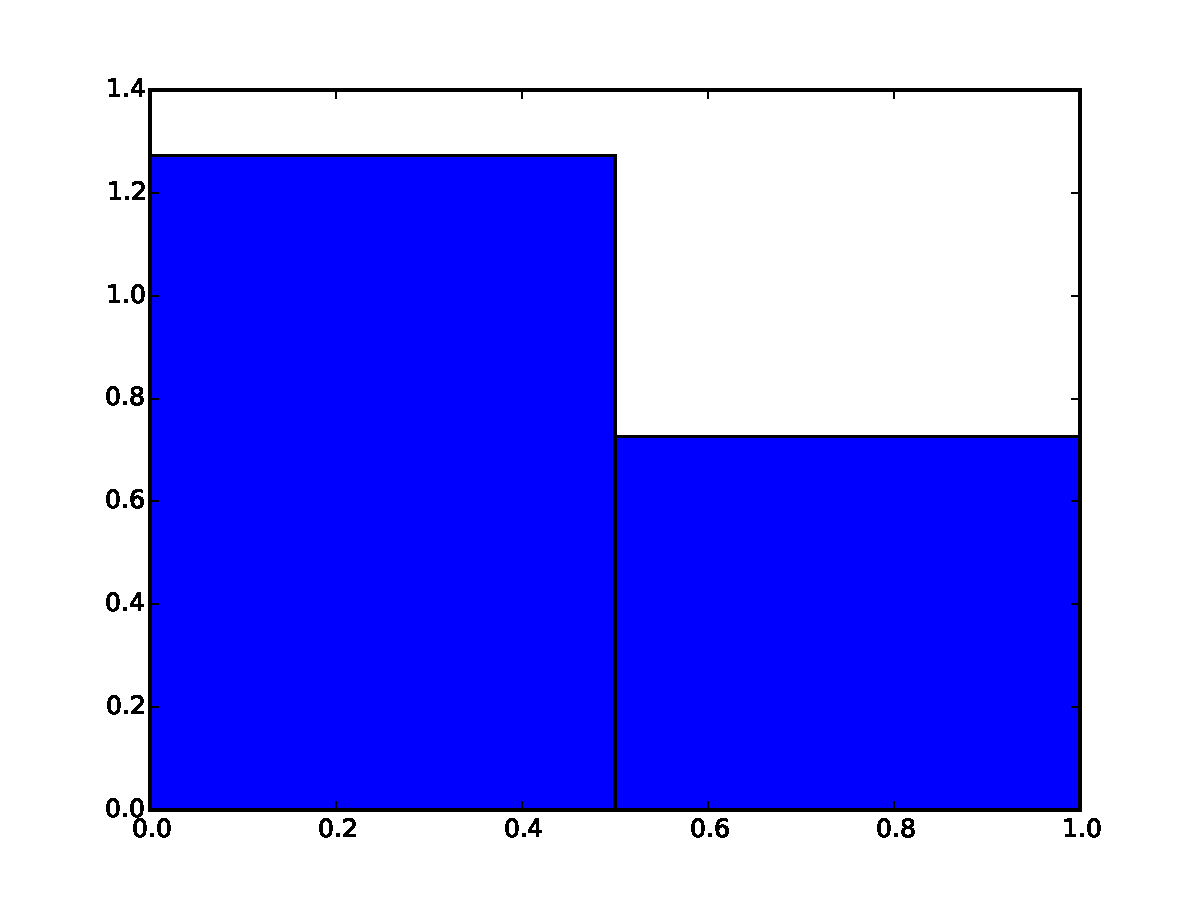
\includegraphics[width=0.5\textwidth]{acc.pdf}
    \caption{Histogram (normalized to a probability density of 1) of acceptance for an MCMC run. 0 is reject, and 1 is accept.}
    \label{fig:acchist}
\end{center}
\end{figure}

Before any analysis can be done on the Markov chain, the ``burn in" steps must be discarded. This can be done quantitatively by looking at the autocorrelation of each parameter and discarding $\sim3$ autocorrelation times. Qualitatively it can be done by simply looking at the $\chi^2$ values. When the chain has ``burned in" the $\chi^2$ values will look like noise around a minimum value. This is shown in Figure \ref{fig:chi}. I chose to discard 20,000 steps of my 300,000 step chain. 

\begin{figure}
\begin{center}
    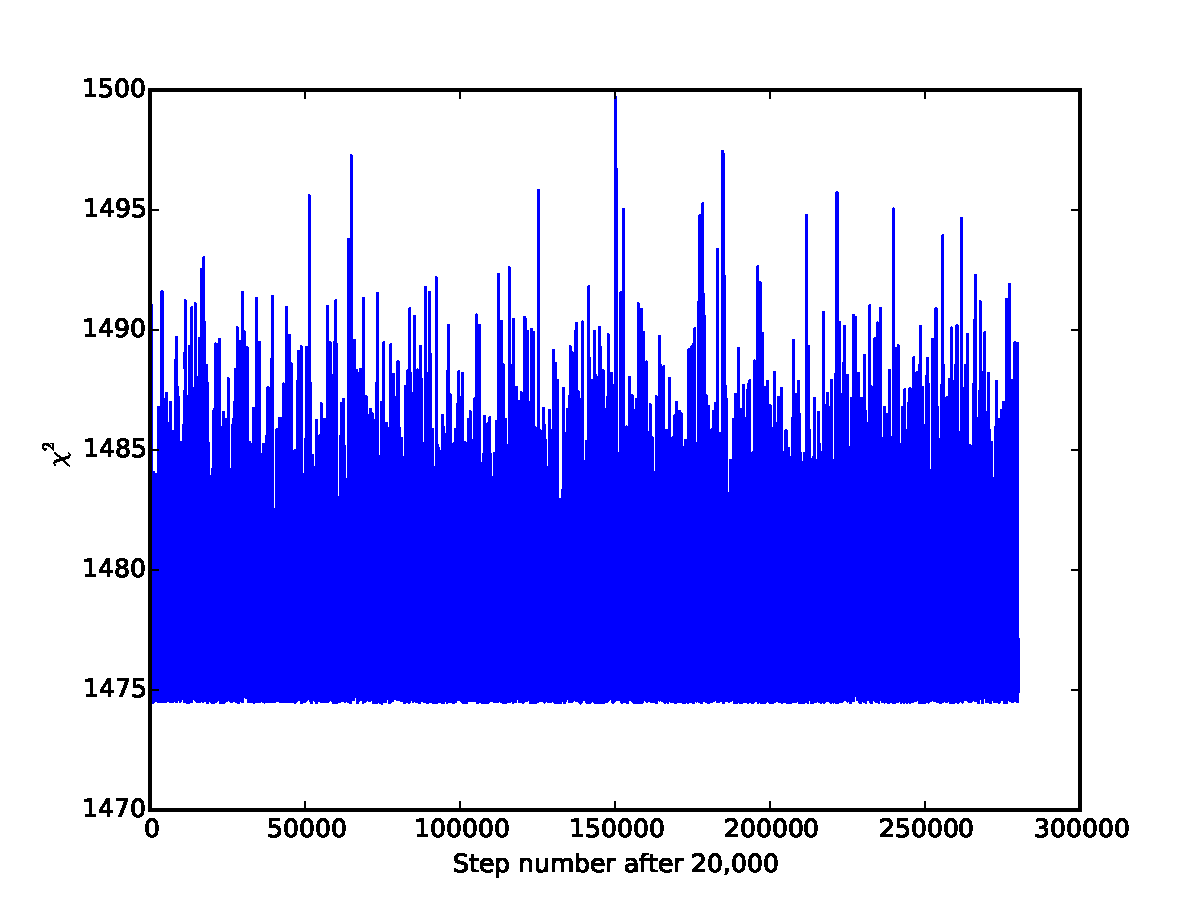
\includegraphics[width=0.6\textwidth]{chiMinusBurn.pdf}
    \caption{$\chi^2$ values after 20,000 steps. There is no downward trend in the values, showing that the chain is fully burned in.}
    \label{fig:chi}
\end{center}
\end{figure}

Median values and $1\sigma$ error bars for the burned in Markov chain are given in Table \ref{tab:bf}. 2D and 1D (marginalized) posterior distributions are shown in Figure \ref{fig:corner}. A phased radial velocity curve showing the data and the best fit model is shown in Figure \ref{fig:rv}. 

\begin{table}
    \begin{center}
        \caption{Orbital Parameters for HD 209458b}\label{tab:bf}
        \begin{tabular}{lc}
            \hline\hline
            Parameter & Median ($1\sigma$) \\
            \hline
            $\tau_0 [\mathrm{HJD}]$ & $2451725.174\pm0.004$ \\
            $P [\mathrm{days}]$ & $3.52468\pm0.00002$ \\
            $M\sin i~[M_J]$ & $0.693\pm0.005$ \\
            \hline
        \end{tabular}
    \end{center}
\end{table}

\begin{figure}
\begin{center}
    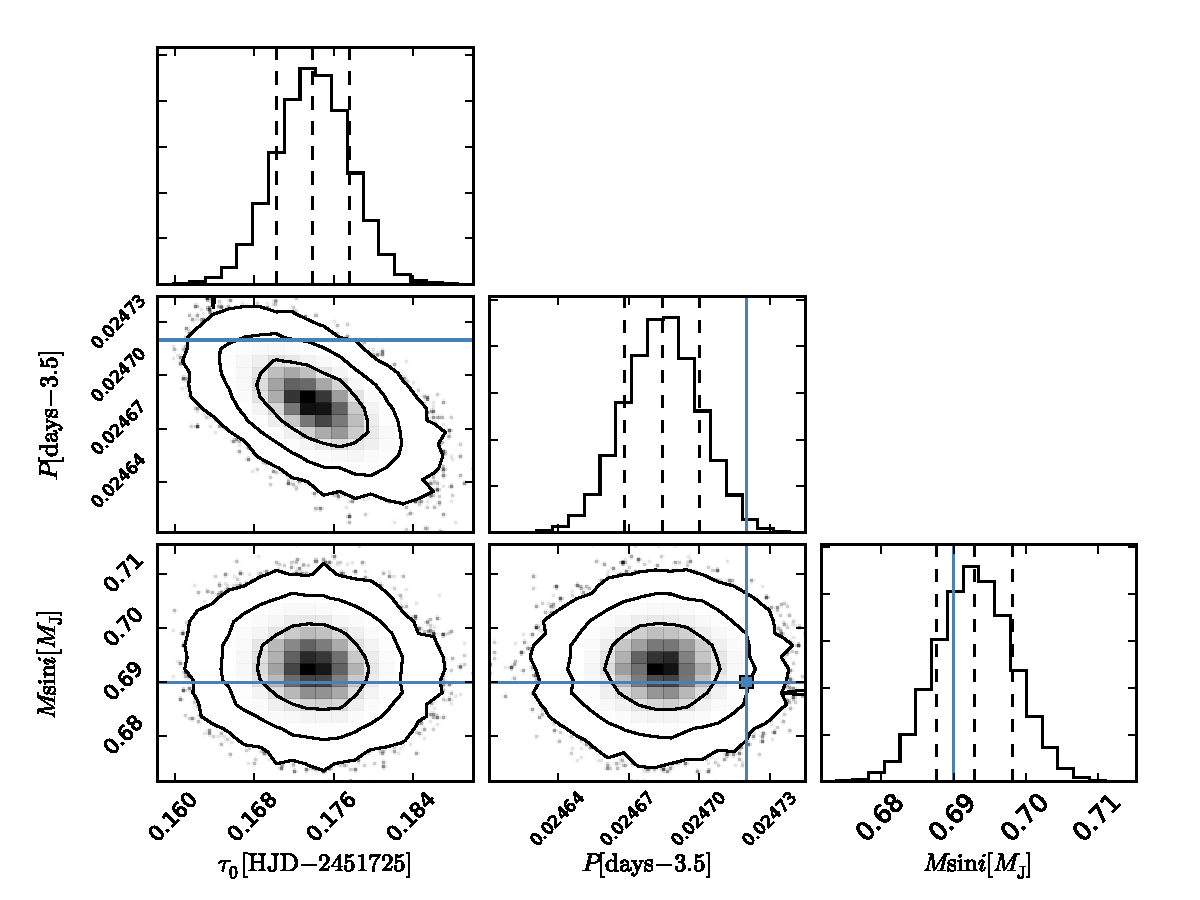
\includegraphics[width=\textwidth]{corner.pdf}
    \caption{Posterior probability distributions for the 3 fitted parameters. Contours are at 67\%, 95\%, and 99.7\%. Dashed lines in the 1D marginalized distributions show the median and 67\% confidence interval. Blue lines show the literature values of $P[\mathrm{days}]=3.52472\pm0.00003$ and $M_p[M_J]=0.69\pm0.02$ \citep{e}.}
    \label{fig:corner}
\end{center}
\end{figure}

\begin{figure}
\begin{center}
    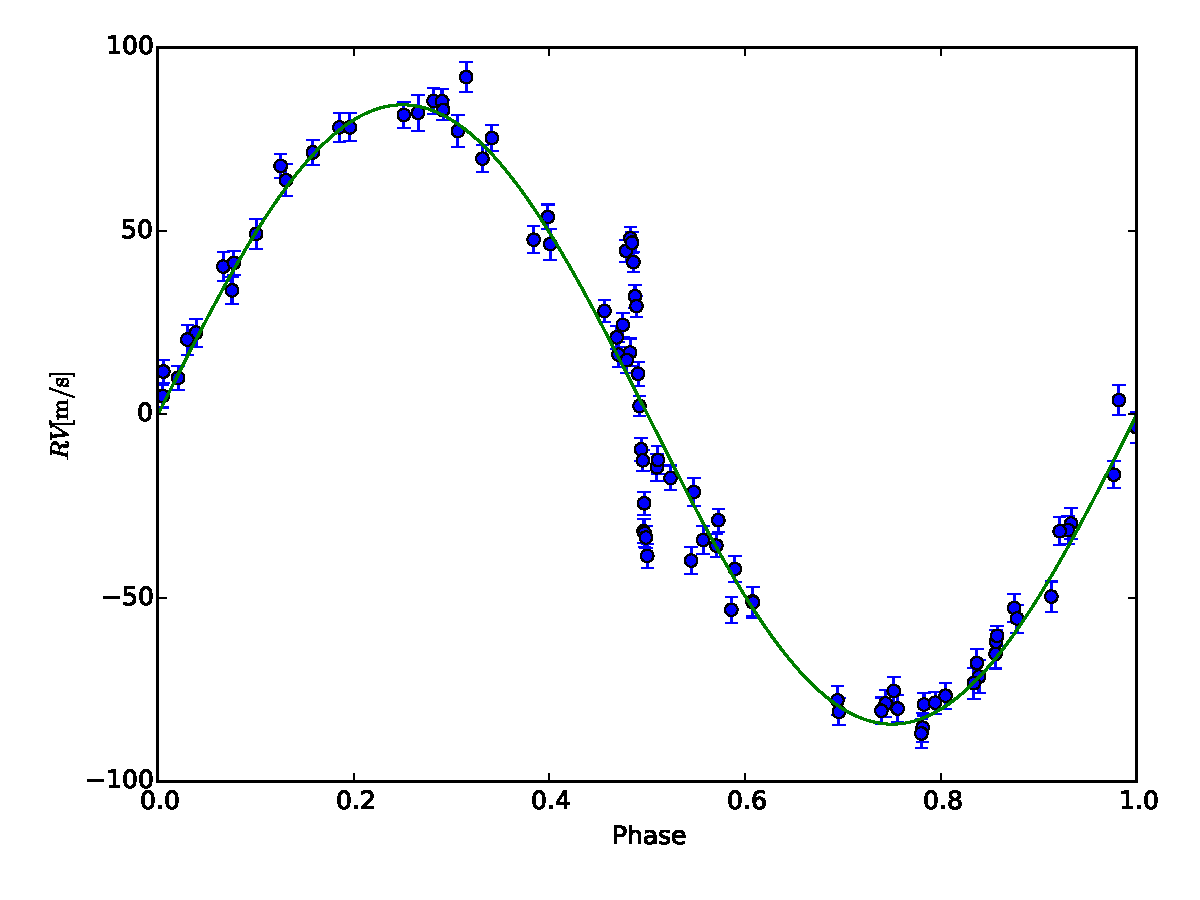
\includegraphics[width=0.6\textwidth]{phrv.pdf}
    \caption{Phased RV curve showing the data and best fit model.}
    \label{fig:rv}
\end{center}
\end{figure}

Something interesting seems to be going on around a phase of 0.5. Upon further investigation, all of these data points are from one epoch (not spread over many phases). This is shown in Figure \ref{fig:err}. This is likely where the slight degeneracy between $\tau_0$ and $P$ is coming from. Since that tight grouping of data points has a lot of leverage on $\chi^2$ locally, shifting the zero point and changing the period accordingly will allow those points to stay near the proposed model. As we have no evidence that these points are anomalous, other than that they qualitatively look off, we cannot exclude them from our analysis. 

Since the anomalies are near a phase of zero, it is possible that these data points are taken during transit and are trying to measure either the atmosphere of the planet or the gas being stripped from it. Again, without confirmation that this is actually what these data points are from (i.e. around the \emph{exact} transit time), I do not feel comfortable excluding them from my fit.

\begin{figure}
\begin{center}
    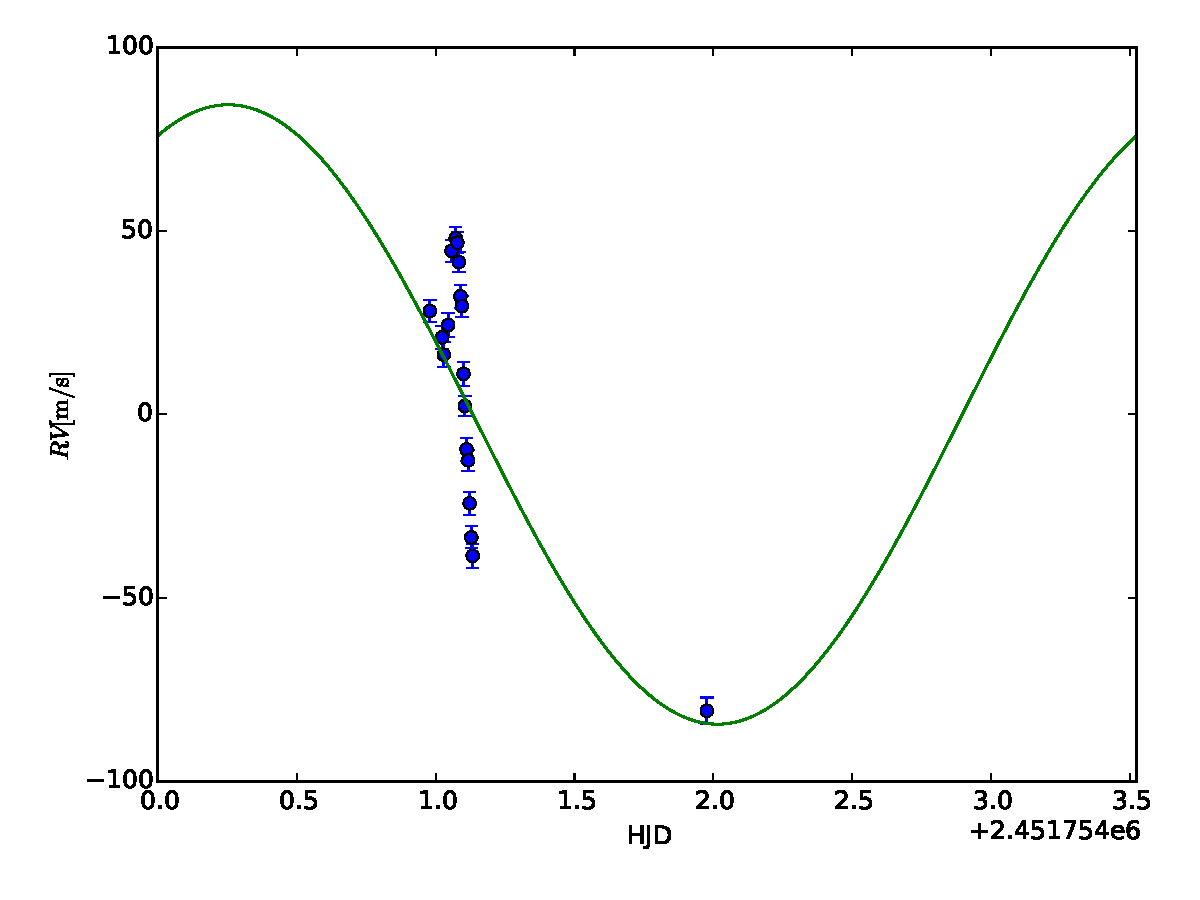
\includegraphics[width=0.6\textwidth]{rverror.pdf}
    \caption{RV curve showing the data and best fit model around the anomalous data points.}
    \label{fig:err}
\end{center}
\end{figure}
%\section{}
%\subsection{}

\setlength\bibsep{0pt}
\bibliographystyle{apj}
\bibliography{sources}

\end{document}  
